\documentclass[11pt]{article}
\usepackage[utf8]{inputenc}
\usepackage[T1]{fontenc}
\usepackage{hyperref}
\usepackage{palatino}
\usepackage{paralist}
\usepackage{verbatim}
\usepackage{amsmath}
\usepackage{graphicx}
\usepackage{footmisc}
\usepackage[a4paper,top=2cm,bottom=2cm,left=2.5cm,right=2.5cm]{geometry}

\makeatletter
\def\verbatim@font{\ttfamily\small}
\makeatother

\usepackage{minted}
\newminted{clojure}{fontsize=\footnotesize,frame=lines,linenos}


\title{Solving the Class Diagram Restructuring Transformation Case with FunnyQT}
\author{Tassilo Horn\\
  \href{mailto:horn@uni-koblenz.de}{horn@uni-koblenz.de}\\
  Institute for Software Technology\\
  University Koblenz-Landau}

\clubpenalty = 10000
\widowpenalty = 10000
\displaywidowpenalty = 10000

%% Reduce the space between image and captions
\setlength\abovecaptionskip{0.2cm}
\setlength\belowcaptionskip{0cm}


\begin{document}

\maketitle

\begin{abstract}
  This paper describes the FunnyQT solution to the TTC 2013 Class Diagram
  Restructuring Transformation Case.

  FunnyQT is a model querying and model transformation library for the
  functional Lisp-dialect Clojure.  It supports the modeling frameworks JGraLab
  and EMF natively, and it is designed to be extensible towards supporting
  other frameworks as well.

  FunnyQT provides a rich and efficient querying API, a model manipulation API,
  and on top of those, there are several sub-APIs for implementing several
  kinds of transformations such as ATL-like model transformations or programmed
  graph transformations.

  This solution tackles the case algorithmically using FunnyQT's plain querying
  and model manipulation APIs.
\end{abstract}

\section{Introduction}
\label{sec:introduction}

\emph{FunnyQT} is a new model querying and transformation approach.  Instead of
inventing yet another language with its own concrete syntax and semantics, it
is implemented as an API for the functional, JVM-based Lisp-dialect
Clojure\footnote{\url{http://clojure.org/}}.  It's JVM-basing provides
wrapper-free access to all existing Clojure and Java libraries, and to other
tools in the rich Java ecosystem such as profilers.

FunnyQT natively supports the de-facto standard modeling framework EMF
\cite{Steinberg2008EEM} and the TGraph modeling framework
JGraLab\footnote{\url{http://jgralab.uni-koblenz.de}}, and it is designed to be
extensible towards other frameworks as well.

FunnyQT's API is split up in several sub-APIs.  On the lowest level there is a
core API for any supported modeling framework providing functions for loading
and storing models, accessing, creating, and deleting model elements, and
accessing and setting attribute values.  These core APIs mainly provide a
concise and expressive interface to the native Java APIs of the frameworks.  On
top of that, there's a generic API providing the subset of core functionality
that is common to both supported frameworks such as navigation via role names,
access to and manipulation of element properties, or functionality concerned
with typing imposed by metamodels.  Furthermore, there is a generic quering API
providing important querying concepts such as quantified expressions, regular
path expressions, or pattern matching.

Based on those querying and model manipulation APIs, there are several sub-APIs
for implementing different kinds of transformations.  For example, there is a
model transformation API similar to ATL \cite{ATL05} or ETL
\cite{booklet:epsilon}, or there is an in-place transformation API for writing
programmed graph transformations similar to GrGen.NET
\cite{manual:GrGenManual}.

Especially the pattern matching API and the transformation APIs make use of
Clojure's Lisp-inherited metaprogramming facilities
\cite{Graham1993OnLisp,Hoyte08LoL} in that they provide macros creating
internal DSLs \cite{book:Fowler2010DSL} providing concise, boilerplate-free
syntaxes to users.  Patterns and transformations written in these internal DSLs
get transformed to usual Clojure code using the FunnyQT querying and model
manipulation APIs by the Clojure compiler.

For solving the tasks of this transformation case\footnote{This FunnyQT
  solution is available at \url{https://github.com/tsdh/ttc-2013-cd-restruct}
  and on SHARE (Section~\ref{sec:run-transformation})\label{fn:github}}, only
FunnyQT's plain querying and model manipulation APIs have been used.


\section{The Core Task}
\label{sec:core-task}

The core task's solution consists of several helper functions, a function for
finding sets of pullable properties and sorting them heuristically in order to
achieve effective results, the three restructuring rules depicted in the case
description \cite{cdrestructcasedesc}, and a last function composing the rules
in order to realized the transformation.  This solution description starts with
the helpers, Section~\ref{sec:restructuring-heuristics} dives into the details
of the function finding pullable properties,
Section~\ref{sec:restructuring-rules} explains the restructuring rules, and
Section~\ref{sec:transf-funct} describes the transformation function.

\subsection{Helper Functions}
\label{sec:helper-functions}

The helper functions discussed in this section are quite simple and factor out
functionality that is used at several places in the rules.

The function \verb|add-prop!| shown in Listing~\ref{lst:add-prop} receives the
single root \verb|model| object \verb|mo|, an \verb|Entity e|, a property name
\verb|pn|, and a \verb|Type t|.  It creates a new \verb|Property p| with the
given name and type, and assigns it to both the given entity and model object.

\begin{listing}[htbp]
  \begin{clojurecode*}{firstnumber=1}
(defn add-prop! [mo e pn t]
  (let [p (ecreate! 'Property)]
    (eadd! mo :propertys p)
    (eset! p :name pn)
    (eset! p :type t)
    (eadd! e :ownedAttribute p)))
  \end{clojurecode*}
  \caption{A function for adding a property to an entity}
  \label{lst:add-prop}
\end{listing}

The \verb|delete-prop!| function depicted in Listing~\ref{lst:delete-prop}
takes an \verb|Entity e|, and a property name \verb|pn|.  It then selects the
\verb|Property p| in the \verb|ownedAttribute| list of \verb|e| which has this
name and deletes it.

\begin{listing}[htbp]
  \begin{clojurecode*}{firstnumber=7}
(defn delete-prop! [e pn]
  (let [p (first (filter #(= pn (eget % :name))
                         (eget e :ownedAttribute)))]
    (edelete! p)
    (eremove! e :ownedAttribute p)))
  \end{clojurecode*}
  \caption{A function for deleting a property from an entity}
  \label{lst:delete-prop}
\end{listing}

The function \verb|pull-up| depicted in Listing~\ref{lst:pull-up} combines
\verb|add-prop!| and \verb|delete-prop!|.  It receives the root \verb|model|
object \verb|mo|, a set of \verb|[propname, type]| tuples \verb|pnts|, a set of
entities \verb|froms| that have these properties, and a single entity
\verb|to|.  For every \verb|[propname, type]| tuple in \verb|pnts|, it creates a new
property in \verb|to|, and deletes the corresponding properties in all
\verb|froms|.

\begin{listing}[htbp]
  \begin{clojurecode*}{firstnumber=12}
(defn pull-up [mo pnts froms to]
  (doseq [[pn t] pnts]
    (add-prop! mo to pn t)
    (doseq [s froms]
      (delete-prop! s pn)))
  true)
  \end{clojurecode*}
  \caption{A function for pulling up properties}
  \label{lst:pull-up}
\end{listing}

Clojure's \verb|doseq| is similar to the \emph{enhanced for loop} in Java, that
is, the elements of an iterable object are bound to a variable one after the
other, and the body is executed for side-effects only.  One interesting
difference visible in line 13 is that \verb|doseq| allows for
\emph{destructuring}.  In Lisp, destructuring means binding the contents of
some structured object directly by imitating the object's structure.  Since
\verb|pnts| is a set of \verb|[propname, type]| tuples, in every iteration the
property name is bound directly to \verb|pn|, and the type is directly bound to
\verb|t|.\footnote{Destructuring is supported by all binding forms including
  \textsf{let}, \textsf{doseq}, \textsf{loop}, the sequence comprehension
  \textsf{for}, and function parameter vectors.}

The next helper, \verb|make-generalization!| shown in
Listing~\ref{lst:make-generalization}, is very simple again.  It creates a new
\verb|Generalization| relationship between an entity \verb|sub| and its
determined superclass \verb|super|.

\begin{listing}[htbp]
  \begin{clojurecode*}{firstnumber=18}
(defn make-generalization! [mo sub super]
  (let [gen (ecreate! 'Generalization)]
    (eadd! mo :generalizations gen)
    (eset! gen :general super)
    (eset! gen :specific sub)))
  \end{clojurecode*}
  \caption{A function for creating a generalization relationship}
  \label{lst:make-generalization}
\end{listing}

The \verb|make-entity!| function is Listing~\ref{lst:make-entity} creates a new
\verb|Entity| and assigns it to the root \verb|model| object \verb|mo|.  Its
name is set to the string ``NewClass'' followed by some number.  \verb|gensym|
is a tool used mostly for metaprogramming.  It returns a guaranteed unique
symbol whose name starts with the given prefix and gets a number appended.
Here, this symbol is just converted to a string.

\begin{listing}[htbp]
  \begin{clojurecode*}{firstnumber=23}
(defn make-entity! [mo]
  (let [e (ecreate! 'Entity)]
    (eadd! mo :entitys e)
    (eset! e :name (str (gensym "NewClass")))))
  \end{clojurecode*}
  \caption{A function for creating an entity}
  \label{lst:make-entity}
\end{listing}

The function \verb|prop-type-set| shown in Listing~\ref{lst:prop-type-set} gets
an \verb|Entity e| and returns its set of \verb|[propname, type]| tuples, i.e.,
there's one such tuple for any owned attribute of \verb|e|.

\begin{listing}[h!tbp]
  \begin{clojurecode*}{firstnumber=27}
(defn prop-type-set [e]
  (set (map (fn [p] [(eget p :name) (eget p :type)])
            (eget e :ownedAttribute))))
  \end{clojurecode*}
  \caption{A function retrieving the set of \textsf{[propname, type]} tuples of
    an entity}
    \label{lst:prop-type-set}
\end{listing}

The standard Clojure higher-order function \verb|map| gets a function and a
collection, and it returns a sequence containing the results of applying that
function to every element of the collection.  \verb|set| then coerces this
sequence to a set.


The \verb|filter-by-properties| function in
Listing~\ref{lst:filter-by-properties} gets a collection of
\verb|[propname, type]| tuples via its \verb|pnts| parameter, and a collection
of entities via its \verb|entities| parameter.  It returns the subset of
\verb|entities|, where every entity defines all of the given properties with
identical types.

\begin{listing}[htbp]
  \begin{clojurecode*}{firstnumber=30}
(defn filter-by-properties [pnts entities]
  (set (filter (fn [e]
                 (forall? #(member? % (prop-type-set e)) pnts))
               entities)))
  \end{clojurecode*}
  \caption{A function for filtering entities to those declaring a given set of
    properties}
  \label{lst:filter-by-properties}
\end{listing}


The syntax \verb|#(member? % (prop-type-set e))| is the shortest form of
defining an anonymous function in Clojure.  The parameters are defined as
\verb|%i| for \verb|i| being
a number larger than 0, and \verb|%| is equivalent
to \verb|%1|.  The largest \verb|i| defines the function's arity.  So here a
local function of arity 1 is defined that checks if its single argument, a
\verb|[propname, type]| tuple, is member of the \verb|prop-type-set| of entity
\verb|e|.


\subsection{Restructuring Heuristics}
\label{sec:restructuring-heuristics}

The rules of this solution don't pull up one attribute at a time, but instead
they pull up the \emph{maximal set of properties that are shared by a maximum
  of entities}.  That is, the heuristics used can be specified as follows.  Let
$P_1$ and $P_2$ be sets of properties shared by the sets of entities $E_1$ and
$E_2$, respectively.

\begin{enumerate}
\item If $|E_1| > |E_2|$, then the solution pulls up the properties of $P_1$
  instead of the properties of $P_2$.  (\emph{Maximality wrt. the number of
    entities declaring these properties})
\item If $|E_1| = |E_2|$, then the solution pulls up the properties of $P_i$
  where~$i = \left\{\begin{array}{ll}1 & \text{if}~|P_1| \geq |P_2|\\2 &
      \text{otherwise}\\ \end{array}\right.$.  (\emph{Maximality wrt. the
    number of pullable properties.})
\end{enumerate}

Figure~\ref{fig:heuristics-example} illustrates these heuristics with two
examples.  In the upper example, the property \verb|c| is shared by three
classes, whereas \verb|a| and \verb|b| are shared by only 2 classes each.  If
the transformation pulls up \verb|a| first into a new class, \verb|c| can be
pulled up only from \verb|C| and \verb|D| into another new class.  The number
of property declaration decreases from 8 to 6, \verb|b| and \verb|c| remain
duplicated once, and 2 new classes have been created.

If the transformation uses the first heuristic, it pulls up \verb|c| first
because that's common to more classes than \verb|a| and \verb|b|.  This also
results in 6 remaining property declarations, \verb|a| and \verb|b| remain
duplicated once, but only one new class has been created.

\begin{figure}[t]
  \centering
  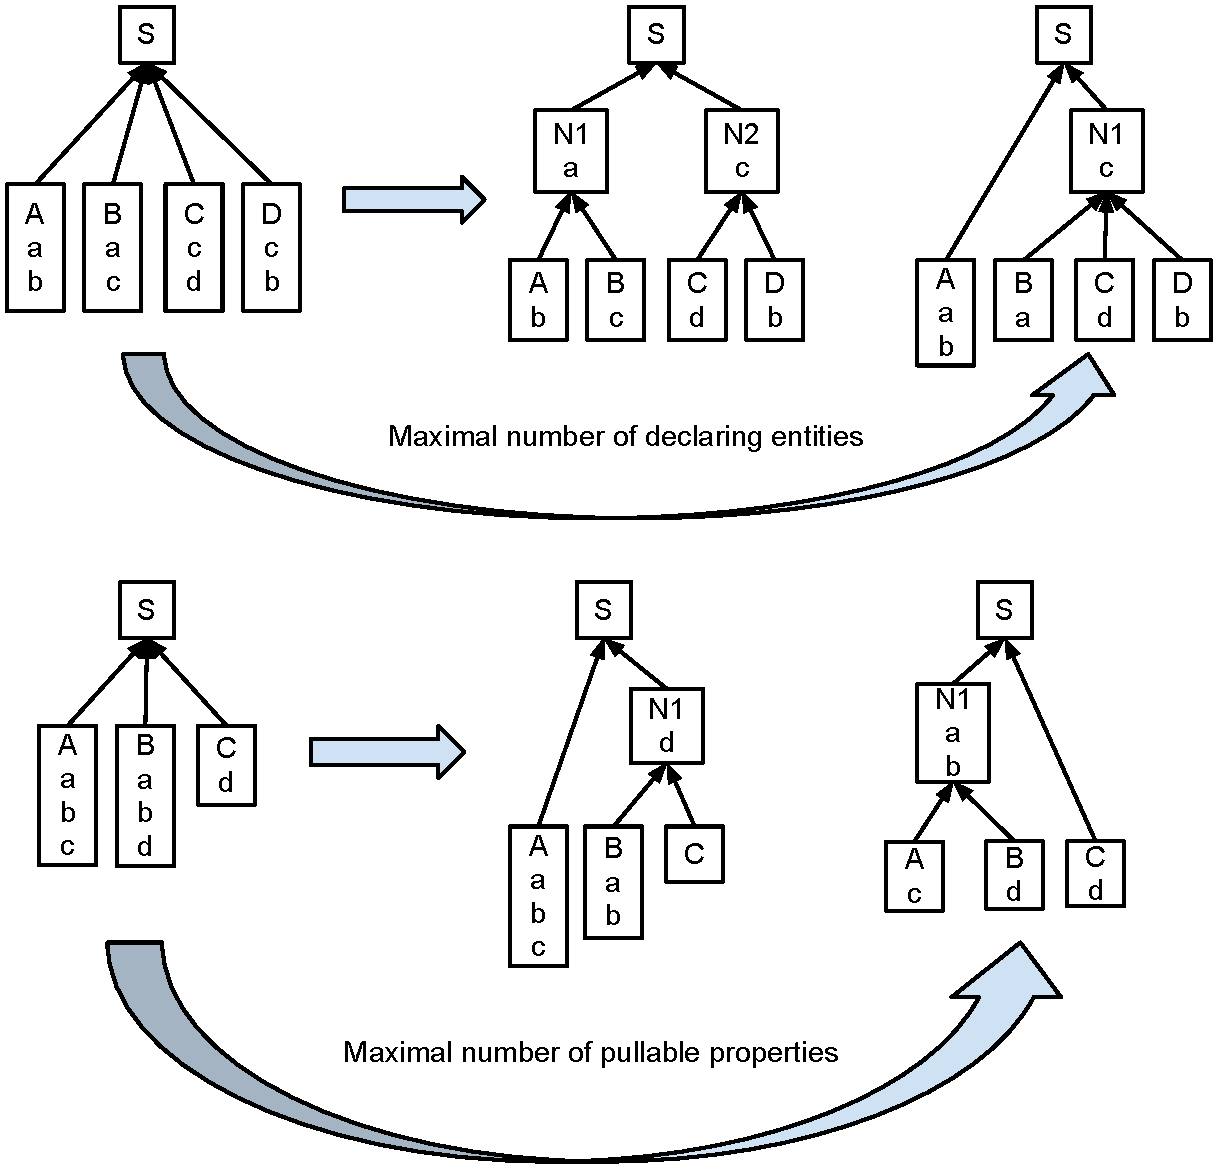
\includegraphics[width=0.6\linewidth]{heuristics-example}
  \caption{Examples for the heuristics}
  \label{fig:heuristics-example}
\end{figure}

In the lower example, the set of properties \verb|{a, b}| and \verb|{d}| are
shared by two classes both.  If the transformation decides to pull up \verb|d|,
the number of property declarations decreases from 7 to 6, \verb|a| and
\verb|b| remain duplicated once, and one new class has been created.

If the transformation uses the second heuristic, it pulls up \verb|a| and
\verb|b|, and the number of property declarations decreases from 7 to 5, only
\verb|d| remains duplicated once, and again one new class has been created.

The \verb|common-props| function for finding sets of pullable properties and
sorting them according to the heuristics is shown in
Listing~\ref{lst:common-props}.  It is by far the most complex function of the
transformation.  The function receives a set of entities via its \verb|classes|
parameter.  The properties common to a maximal subset of these entities are to
be found.

\begin{listing}[b!]
  \begin{clojurecode*}{firstnumber=34}
(defn common-props [classes]
  (let [pes (set (map (fn [pnt]
                        [pnt (filter-by-properties [pnt] classes)])
                      (set (mapcat prop-type-set classes))))
        freq-map (apply hash-map
                        (mapcat (fn [[_ ents]]
                                  [ents (count (filter #(= ents (second %))
                                                       pes))])
                                pes))
        collapse (fn collapse [aes]
                   (when-let [[pnt entities] (first aes)]
                     (let [[s r] (split-with (fn [[_ ents]]
                                               (= entities ents)) aes)]
                       (cons [(map first s) entities]
                             (lazy-seq (collapse r))))))]
    (collapse (into (sorted-set-by
                     (fn [[_ aes :as a] [_ bes :as b]]
                       (let [x (- (count bes) (count aes))]
                         (if (zero? x)
                           (let [x (- (freq-map bes) (freq-map aes))]
                             (if (zero? x)
                               (compare a b)
                               x))
                           x))))
                    pes))))
  \end{clojurecode*}
  \caption{A function for retrieving the maximal set of properties shared by a
    maximum of classes}
  \label{lst:common-props}
\end{listing}

In line 35, the variable \verb|pes| is bound to a set of the following
form\footnote{\textsf{\#\{...\} is a Clojure set literal.}}.

\begin{clojurecode*}{linenos=none}
#{[[pn1 t1] #{e1 e2 e3}]
  [[pn4 t2] #{e2 e3 e4}]
  [[pn2 t2] #{e2 e3 e4 e5}]
  [[pn3 t2] #{e1 e2 e3}]}
\end{clojurecode*}

I.e., the set's items are tuples where the first component is a
\verb|[propname, type]| tuple, and the second component is the set of entities
declaring this property.  There is exactly one item for every unique pair of
property name and type.

In line 38, \verb|freq-map| is bound to a hash-map that maps to each set of
entities occuring in the items of \verb|pes| the number of occurences in there.
This map will be used to implement the second heuristic.

In line 43, a local function \verb|collapse| is defined.  Before explaining
that, first lines 49 to 58 are to be explained.  What's done there is that the
entries of the set \verb|pes| are put into a sorted set.  The sorting order is
determined by the comparator function defined in lines 50 to 57.  It's meaning
is equivalent to comparator objects in Java.  It gets two objects and returns a
negative number if the first object should be sorted before the second, it
returns a positive number if the second object should be sorted before the
first one, and it returns zero if both objects are equal.

Here, the comparator function receives two items of the \verb|pes| set.  It
uses destructuring to bind the first one to \verb|a| and its entity set to
\verb|aes|.  The first component of each item, the \verb|[propname, type]|
tuple, is ignored.  Similarly, the second item is bound to \verb|b| and its set
of entities is bound to \verb|bes|.  The comparator function then performs
these checks:

\begin{enumerate}
\item If \verb|bes| contains more entities than \verb|aes|, \verb|b| should be
  sorted before \verb|a|.  This implements heuristic 1.
\item Else, if the entity set \verb|bes| occurs more often in the items of
  \verb|pes|, \verb|b| should be sorted before \verb|a|.  This implements
  heuristic 2.
\item Else the sorting order is not important and determined by Clojure's
  standard \verb|compare| function that produces a stable ordering upon all
  objects implementing \verb|Comparable|.
\end{enumerate}

As a result, the sorted set has the following structure.

\begin{clojurecode*}{linenos=none}
#{[[pn2 t2] #{e2 e3 e4 e5}]
  [[pn1 t1] #{e1 e2 e3}]
  [[pn3 t2] #{e1 e2 e3}]
  [[pn4 t2] #{e2 e3 e4}]}
\end{clojurecode*}

Items with larger entity sets are sorted before items with smaller entity sets,
e.g., the item with \verb|pn2| is sorted before the others because it is shared
by 4 entities.  In case of equally large entity sets, the number of occurences
of the entity sets determines the sorting order, e.g., the items with
\verb|pn1| and \verb|pn2| are sorted before the item with \verb|pn4|, because
their entity sets occur twice whereas the entity set of \verb|pn4| occurs only
once.

Finally, this set is mangled by the local \verb|collapse| function.  When the
provided sorted set \verb|aes| contains a first entry (line 44), the set is
split in two parts \verb|s| and \verb|r|, where \verb|s| contains all the items
that have the very same entities set as the first item.  The result of the
function is a list\footnote{In fact, the result is no list but a lazy sequence
  because the recursive call is wrapped with \textsf{lazy-seq}.  A lazy seq is
  similar to a list, but the elements in its rest are not computed
  (\emph{realized}) before someone tries to access them.  That is, the rest of
  a lazy sequence is actually a closure that knows how to realize the sequence
  one step further.}  where the head is a tuple \verb|[pnts entities]|, where
\verb|pnts| is a list of \verb|[propname, type]| tuples, and the rest is the
result of applying \verb|collapse| to the split-off part \verb|r|.  Using the
example again, the result structure is as follows.

\begin{clojurecode*}{linenos=none}
([([pn2 t2])          #{e2 e3 e4 e5}]
 [([pn1 t1] [pn3 t2]) #{e1 e2 e3}]
 [([pn4 t2])          #{e2 e3 e4}]}
\end{clojurecode*}

That is, neighboring items with equal entity sets are collapsed into one.


\subsection{Restructuring Rules}
\label{sec:restructuring-rules}

In this section, the three restructuring rules are explained.  With the
\verb|common-props| function in place, some observations can be made.  Rule 1
and rule 2 are nearly identical.  When looking for shared properties in a set
of subclasses, if there are properties shared by all of them, this is of course
the maximal set, too.  The only difference is that for rule 1, no new entity
has to be created, while for rule 2, where only a subset of subclasses shares
properties, a new entity has to be created.

Also rule 2 and rule 3 are very similar.  The difference is only if common
properties are searched below subclasses of a given class, or below top-level
classes.

Therefore, the solution defines the function \verb|pull-up-helper| shown in
Listing~\ref{lst:pull-up-helper} which can implement all rules by
parameterizing it appropriately.  The function receives the root \verb|model|
object \verb|mo|, a superclass \verb|super|, and a set of entities
\verb|classes| in which to find common properties,.  In case of rule 1 and rule
2, \verb|super| is the superclass of all \verb|classes|, and in case of rule 3,
the \verb|super| parameter is \verb|nil| and \verb|classes| is the set of
top-level classes.

\begin{listing}[htbp]
  \begin{clojurecode*}{firstnumber=59}
(defn pull-up-helper [mo super classes]
  (when (seq classes)
    (when-let [[pnts entities] (first (common-props classes))]
      (if (and super (= classes entities))
        (pull-up mo pnts entities super)  ;; rule 1
        (when (> (count entities) 1)
          (let [nc (make-entity! mo)]     ;; rule 2 if super, else rule 3
            (pull-up mo pnts entities nc)
            (doseq [s entities]
              (doseq [oldgen (eget s :generalization)
                      :when (= super (adj oldgen :general))]
                (edelete! oldgen))
              (make-generalization! mo s nc))
            (when super (make-generalization! mo nc super))
            true))))))
  \end{clojurecode*}
  \caption{A restructuring function able to implement all three rules}
  \label{lst:pull-up-helper}
\end{listing}

When the set of classes is not empty\footnote{\textsf{(seq coll)} is the
  canonical non-emptyness check in Clojure.} (line 60), and if there are common
properties, the largest list of common properties among the lists of properties
declared by a maximal number of entities is bound to \verb|pnts|, and the
entities declaring these properties are bound to \verb|entities| (line 61).

In case \verb|entities| equals the set of all \verb|classes| (line 62), the
situation is that of rule 1, and all properties in \verb|pnts| are pulled up to
\verb|super| (line 63).

In the other case, the maximal set of common properties is shared by a maximal
but real subset of \verb|classes|.  In that case, it has to be ensured that
there are more than one entity declaring these properties (line 64), because
else the inheritance depth would increase without removing declarations.

Then, the situation is that of rule 2 if \verb|super| is non-nil, or the
situation is that of rule 3 if \verb|super| is nil.  In any case, a new entity
\verb|nc| has to be created (line 65), and all properties \verb|pnts| have to
be pulled from \verb|entities| to \verb|nc| (line 66).  The original
generalizations to \verb|super| are deleted (lines 67 to 70), and new
generalizations from the entities to \verb|nc| are created (line 71).

If \verb|super| is non-nil, also a new generalization from \verb|nc| to the
original superclass \verb|super| is created (line 72).  Finally, \verb|true| is
returned to indicate to the caller that a restructuring has performed.

Using this helper, the individual rules are very easy.
Listing~\ref{lst:pull-up-1-2} shows the function implementing rule 1 and 2.  It
uses \verb|loop|/\verb|recur|, a local tail-recursion, to call the
\verb|pull-up-helper| once for any class and its subclasses.  The
\verb|applied| variable determines the return value of the function.  It is
\verb|true| if the helper could perform a restructuring at least once.


\begin{listing}[htbp]
  \begin{clojurecode*}{firstnumber=74}
(defn pull-up-1-2 [mo]
  (loop [classes (eget mo :entitys), applied false]
    (if (seq classes)
      (let [super (first classes)
            result (pull-up-helper
                    mo super (set (adjs super :specialization :specific)))]
        (recur (rest classes) (or result applied)))
      applied)))
  \end{clojurecode*}
  \caption{A function applying rule 1 and 2 to all classes}
    \label{lst:pull-up-1-2}
\end{listing}

Listing~\ref{lst:pull-up-3} depicts the function \verb|pull-up-3| implementing
rule 3.

\begin{listing}[htbp]
  \begin{clojurecode*}{firstnumber=82}
(defn pull-up-3 [mo]
  (pull-up-helper mo nil (set (remove #(seq (eget % :generalization))
                                      (eget mo :entitys)))))
  \end{clojurecode*}
  \caption{A function applying rule 3 to all top-level classes}
    \label{lst:pull-up-3}
\end{listing}

It simply calls the helper providing \verb|nil| as superclass parameter, and
the set of top-level classes.


\subsection{The Transformation Function}
\label{sec:transf-funct}

The function \verb|pull-up-attributes| shown in
Listing~\ref{lst:pull-up-attributes} implements the overall transformation by
calling the rules defined in the previous section.  It receives the class
diagram EMF model via its \verb|model| parameter, and the
\verb|multi-inheritance| parameter specifies if multiple inheritance should be
exploited in order to minimize the number of property declarations.  This
extension task is discussed in Section~\ref{sec:extension-task}.

\begin{listing}[htbp]
  \begin{clojurecode*}{firstnumber=85}
(defn pull-up-attributes [model multi-inheritance]
  (let [mo (the (eallobjects model 'model))]
    (iteratively #(let [r (pull-up-1-2 mo)]
                    (or (pull-up-3 mo) r)))
    (when multi-inheritance (exploit-multiple-inheritance mo))
    model))
  \end{clojurecode*}
  \caption{The transformation function}
    \label{lst:pull-up-attributes}
\end{listing}

In line 86, the single root \verb|model| object is retrieved and bound to the
variable \verb|mo|.  The function \verb|iteratively| in line 87 takes a
function and applies it as long as it returns \verb|true|.  The anonymous
function given to it first applies the \verb|pull-up-1-2| rule, then the
\verb|pull-up-3| rule.  It returns \verb|true| if at least one of the rules
could be applied.

In case \verb|multi-inheritance| is \verb|true|, another rule which is
explained in Section~\ref{sec:extension-task} is applied.  Finally, the
\verb|model| is returned.



\section{The Multiple Inheritance Extension Task}
\label{sec:extension-task}

The rules discussed in Section~\ref{sec:restructuring-rules} work well also if
the initial model already contains multiple inheritance.  However, they won't
create new classes that specialize more than one single superclass.

To exploit the presence of multiple inheritance in order to restructure the
model resulting from the core rules so that every property is declared exactly
once, the additional rule shown in
Listing~\ref{lst:exploit-multiple-inheritance} is used.  It receives the root
\verb|model| object as its only parameter.

\begin{listing}[htbp]
  \begin{clojurecode*}{firstnumber=90}
(defn exploit-multiple-inheritance [mo]
  (doseq [[pnts entities] (common-props (eget mo :entitys))
          :while (> (count entities) 1)]
    (let [[nc reuse]
          (if-let [top (first (filter
                               #(and (empty? (eget % :generalization))
                                     (re-matches #"NewClass.*" (eget % :name)))
                               entities))]
            [top true]
            [(make-entity! mo) false])]
      (doseq [[pn t] pnts]
        (when-not reuse
          (add-prop! mo nc pn t))
        (doseq [e (remove #(= nc %) entities)]
          (delete-prop! e pn)
          (make-generalization! mo e nc))))))
  \end{clojurecode*}
  \caption{A function for exploiting multiple inheritance}
    \label{lst:exploit-multiple-inheritance}
\end{listing}

\begin{sloppypar}
  The function iterates over the result list of common properties of all
  entities in the model that are shared by at least 2 entities.  In every
  iteration, \verb|pnts| is bound to a list of \verb|[propname type]| tuples,
  and \verb|entities| is the set of entities declaring these properties.
\end{sloppypar}

Naively, one could create a new entity in every iteration, pull the common
properties into it, and make all \verb|entities| subclasses of the new one.
But this might create more new entities than necessary.  Instead, it is
preferrable to reuse some existing top-level class that already declares these
properties.  In that case, only new generalizations have to be created from all
\verb|entities| (except this one) to this top-level class, and the shared
properties have to be deleted from the subclasses.

The function takes into account one further issue.  When looking for such a
top-level class, only the classes created by the rules of the core task are
considered.  The reason is that reusing an entity that already existed in the
original class model will make the transformation result's type hierarchy
incompatible with that of the original model, that is, in the original model
\verb|B| was no subclass of \verb|A|, but in the result model it is.  Such a
change is likely to break programs implemented using these classes since its
polymorphic method calls and instance tests might deliver unexpected results.



\section{Running the Transformation on SHARE}
\label{sec:run-transformation}

The FunnyQT solution to this case\footref{fn:github} (and the other cases) are
installed on the SHARE image \verb|Ubuntu12LTS_TTC13::FunnyQT.vdi|.  Running
the solution is simple.

\begin{compactenum}
\item Open a terminal.
\item Change to the Class Diagram Restructuring project:

  \verb|$ cd ~/Desktop/FunnyQT_Solutions/ttc-2013-cd-restruct/|
\item To run the transformation for all provided and some additional but small
  models, use:

  \verb|$ lein test|

  This will run the complete transformation on all provided and some additional
  test models and print the execution times.  For every model, the core task
  transformation and also the multiple inheritance enabled transformation is
  performed.

  \begin{sloppypar}
    The result models are also validated using unit tests defined in the file
    \verb|test/ttc_2013_cd_restruct/core_test.clj|.  The result models and
    visualizations are saved to the \verb|results| directory.
  \end{sloppypar}
\item To determine the maximum capability of the solution, some more variants
  of test case 2 have been generated.  Here the model sizes are 500000,
  1000000, and 2000000 elements.  To apply the transformation to these models,
  use:

  \verb|$ lein test :stress|

  The maximum capability (on SHARE) is the largest model with 2 million
  elements.  To apply the transformation to only this model, use:

  \verb|$ lein test :maximum|

  Running the tests with \verb|:maximum| will take about 40 minutes, and
  running the tests with \verb|:stess| will take about an hour.
\end{compactenum}


\section{Evaluation}
\label{sec:evaluation}

The evaluation results requested by the case description
\cite{cdrestructcasedesc} are summarized in Table~\ref{tab:evaluation}.

With respect to \emph{size}, the FunnyQT solution to the core task consists of
exactly 90 lines of code excluding comments, empty lines, and namespace
declarations.  The extension rule for exploiting multiple inheritance accounts
for another 15 LOCs.  This seems quite good, although the UML-RSDS reference
solution is only about 30 LOCs due to its very declarative nature.

The case description defines the \emph{complexitiy} as the sum of operator
occurences, type references, and feature references.  The FunnyQT solution
consists of 161 function calls (or calls to special forms or macros), 4 type
references, and 25 feature references.

For all provided test models, the \emph{effectiveness} of the core task
solution is 100\%.  The unit tests also apply the core transformation to
several additional models (such as the ones depicted in
Figure~\ref{fig:heuristics-example}) in which the implemented heuristics are of
importance.  For these models, the effectiveness is 100\%, too.  When the
transformation including the multiple inheritance rule is applied to the
models, the result is that every duplication is removed, i.e., every property
is declared exactly once.

The \emph{development effort} is quite hard to estimate retrospectively,
because it has been an on-off task.  The initial working version for the core
task has been implemented from scratch in about two hours.  After thinking
about it in my spare time and restructuring some more sample models using pen
and paper, it has been refactored and enhanced to the solution presented in
this paper.  All in all, a development effort of approximately 8 hours seems
realistic.  About two additional hours have been invested for defining the unit
tests.

\begin{table}[htb]
  \centering
  \begin{tabular}{| l | l |}
    \hline
    \textbf{Measure}            & \textbf{Value}\\
    \hline
    \textbf{Size (LOC)}         & 90 (core only), 105 (core + extension)\\
    \textbf{Complexity}         & 190 = 161 funcalls + 4 type refs + 25 feature refs\\
    \textbf{Effectiveness}      & 100\%\\
    \textbf{Development effort} & approx. 8 hours (solution) + 2 hours (tests)\\
    \textbf{Execution time}     & 6 secs for the largest model (\verb|testcase2_10000.xmi|)\\
    \textbf{History of use}     & approx. 1 year\\
    \textbf{Maximum capability} & approx. 2 million elements on SHARE\\
    \hline
  \end{tabular}
  \caption{Evaluation measures}
  \label{tab:evaluation}
\end{table}

The detailed \emph{execution times} rounded to whole milliseconds on SHARE for
all provided models are depicted in Table\ref{tab:exec-times}.  The largest
provided model consisting of 100000 elements\footnote{The models
  \textsf{testcase2\_n} actually consist of $10\times n$ elements.} can be
processed in about six seconds which is more than a thousand times faster than
the reference UML-RSDS solution.  It can be seen that the additional multiple
inheritance rule has only little influence on the execution times.

\begin{table}[htb]
  \centering
  \begin{tabular}{| l | r | r |}
    \hline
    \textbf{Provided model}    & \textbf{Core task only} & \textbf{Core and Extension task}\\
    \hline
    \textsf{testcase1}         & 1 ms      & 1 ms\\
    \textsf{testcase2}         & 1 ms      & 1 ms\\
    \textsf{testcase2\_1000}   & 418 ms    & 434 ms\\
    \textsf{testcase2\_5000}   & 2455 ms   & 2585 ms\\
    \textsf{testcase2\_10000}  & 5656 ms   & 6041 ms\\
    \textsf{testcase3}         & 248 ms    & 268 ms\\
    \hline
    \textsf{mitest1}           & 1 ms      & 1 ms\\
    \textsf{mitest2}           & 1 ms      & 1 ms\\
    \textsf{mitest3}           & 1 ms      & 1 ms\\
    \hline
    \textbf{Additional model}  & & \\
    \hline
    \textsf{testcase2\_50000}  & 75238 ms  & 76835 ms\\
    \textsf{testcase2\_100000} & 262917 ms & 264483 ms\\
    \textsf{testcase2\_200000} & 1006848 ms & 1045648 ms\\
    \hline
  \end{tabular}
  \caption{Detailed execution times on SHARE}
  \label{tab:exec-times}
\end{table}

\begin{sloppypar}
  To determine the \emph{maximum capability} of the solution, the models
  \verb|testcase2_50000|, \verb|testcase2_100000|, and \verb|testcase2_200000|
  consisting of half a million, one million, and two million elements,
  respectively, have been generated.  Transforming \verb|testcase2_50000| runs
  slightly more than one minute, \verb|testcase2_100000| runs in about five
  minutes, and \verb|testcase2_200000| runs in about 17 minutes.  Given the
  limited amount of 800 MB memory available to the JVM process on SHARE, the
  model with 2 million elements is approximately the maximum capability for the
  FunnyQT solution.
\end{sloppypar}


\bibliographystyle{alpha}
\bibliography{ttc13-funnyqt-cd-restruct}


\end{document}




%%% Local Variables:
%%% mode: latex
%%% TeX-engine: pdflatex-shell-escape
%%% TeX-master: t
%%% End:
